\documentclass[12pt, a4paper]{article}
\usepackage[utf8]{inputenc}
\usepackage{amsmath}
\usepackage{amsthm}
\usepackage{amssymb}
\usepackage{graphicx}
\usepackage{parskip}
\usepackage{hyperref}
\usepackage{fancyhdr}
\usepackage{lastpage}
\usepackage[vlined,ruled]{algorithm2e}
\usepackage[acronym]{glossaries}
\usepackage{caption}
\usepackage{titlesec}
\usepackage{tikz}
\usetikzlibrary{arrows,automata}

\titleformat{\section}
  {\normalfont\bfseries}{Problem 6.\thesection}
  {0em}{}

\titleformat{\subsection}
  {\normalfont\bfseries}{6.\thesubsection}
  {0em}{}

\titleformat{\subsubsection}
  {\normalfont\bfseries}{6.\thesubsection}
  {0em}{}

\title{%
  Stochastic Network Modeling \\
  Homework 6 - Solutions
}
\author{%
  Juan Pablo Royo Sales\\
  \small{Universitat Politècnica de Catalunya}
}
\date\today

\pagestyle{fancy}
\fancyhf{}
\fancyhead[C]{}
\fancyhead[R]{Juan Pablo Royo Sales - UPC MIRI}
\fancyhead[L]{SNM - Homework 6}
\fancyfoot[L,C]{}
\fancyfoot[R]{Page \thepage{} of \pageref{LastPage}}
\setlength{\headheight}{15pt}
\renewcommand{\headrulewidth}{0.4pt}
\renewcommand{\footrulewidth}{0.4pt}

\renewcommand{\qedsymbol}{$\blacksquare$}

\begin{document}

\maketitle

\section{}
\subsection{}
\begin{subequations}
  \begin{align}
    f_{ss} &= p_{ss} + p_{sc}f_{ss}\\
           &= 0.9 + 0.1 f_{ss}\\
           &= \frac{0.9}{1-0.1}\\
           &= 1
  \end{align}
\end{subequations}


\begin{subequations}
  \begin{align}
    f_{cc} &= p_{cc} + p_{cs}f_{cc}\\
           &= 0.8 + 0.2 f_{cc}\\
           &= \frac{0.8}{1-0.2}\\
           &= 1
  \end{align}
\end{subequations}


\subsection{}

\begin{subequations}
  \begin{align}
    m_{ss} &= p_{ss} + p_{sc}(1 + m_{ss})\\
           &= 0.9 + 0.1  + 0.1 m_{ss}\\
           &= \frac{1}{1-0.1}\\
           &= 1.11
  \end{align}
\end{subequations}


\begin{subequations}
  \begin{align}
    m_{cc} &= p_{cc} + p_{cs}(1 + m_{cc})\\
           &= 0.8 + 0.2  + 0.2 m_{cc}\\
           &= \frac{1}{1-0.2}\\
           &= 1.25
  \end{align}
\end{subequations}

\section{}
\begin{subequations}
  \begin{align}
    f_{4w} &= p_{4w} + p_{44}f_{4w} + p_{45}f_{4w} + p_{46}f_{4w}\\
           &= \frac{3}{36} + \frac{27}{36}f_{4w} + 0 + 0 \\
           &= \frac{1}{3}
  \end{align}
\end{subequations}


\begin{subequations}
  \begin{align}
    f_{5w} &= p_{5w} + p_{55}f_{5w} + p_{54}f_{5w} + p_{56}f_{5w}\\
           &= \frac{4}{36} + \frac{26}{36}f_{5w} + 0 + 0 \\
           &= \frac{2}{5}
  \end{align}
\end{subequations}

\begin{subequations}
  \begin{align}
    f_{6w} &= p_{6w} + p_{66}f_{6w} + p_{65}f_{6w} + p_{64}f_{6w}\\
           &= \frac{5}{36} + \frac{25}{36}f_{6w} + 0 + 0 \\
           &= \frac{5}{11}
  \end{align}
\end{subequations}

Probability of wining is
\begin{subequations}
  \begin{align}
    P(\text{wining}) &= (1-f_{ll}) * f_{ww} * f_{4w} * f_{5w} * f_{6w}\\
                     &= (1-\frac{4}{36}) * \frac{8}{36} * \frac{1}{3} * \frac{2}{5} * \frac{5}{11}
                     &= \frac{32}{2673}\\
                     &= 0.01
  \end{align}
\end{subequations}

\section{}
\subsection{}
First lets do the $f_{i(HH)}$
\begin{subequations}
  \begin{align}
    f_{H(HH)} &= p_{H(HH)} + p_{H(T)} f_{T(HH)}\\
              &= \frac{1}{2} + \frac{1}{2} f_{T(HH)}\label{eq:1}
  \end{align}
\end{subequations}

\begin{subequations}
  \begin{align}
    f_{(TT)(HH)} &= p_{(TT)(HH)} + p_{(TT)(TTT)}f_{(TTT)(HH)} + p_{(TT)(H)} f_{H(HH)}\\
                 &= 0 + 0 + \frac{1}{2} (\frac{1}{2} + \frac{1}{2} f_{T(HH)})\\
                 &= \frac{1}{4} + \frac{1}{4} f_{T(HH)} \label{eq:2}
  \end{align}
\end{subequations}

\begin{subequations}
  \begin{align}
    f_{T(HH)} &= p_{T(HH)} + p_{TH}f_{H(HH)} + p_{T(TT)} f_{(TT)(HH)}\\
              &= 0 + 0 + \frac{1}{2} (\frac{1}{2} + \frac{1}{2} f_{T(HH)}) + \frac{1}{2} f_{(TT)(HH)}\\
              &= \frac{1}{4} + \frac{1}{4} f_{T(HH)} + \frac{1}{2} f_{(TT)(HH)}\\
              &= \frac{1}{4} + \frac{1}{4} f_{T(HH)} + \frac{1}{2} (\frac{1}{4} + \frac{1}{4} f_{T(HH)})\label{eq:3}\\
              &= \frac{1}{4} + \frac{1}{4} f_{T(HH)} + \frac{1}{8} + \frac{1}{8} f_{T(HH)}\\
              &= \frac{3}{8} + \frac{3}{8} f_{T(HH)}\\
              &= \frac{3}{5}\label{eq:4}
  \end{align}
\end{subequations}


Here~\ref{eq:3} plugin~\ref{eq:2}

Now applying~\ref{eq:4} into~\ref{eq:2} we have that $f_{(TT)(HH)} = \frac{2}{5}$.

And also applying~\ref{eq:4} into~\ref{eq:1} we have that $f_{H(HH)} = \frac{4}{5}$.

\subsection{}
Now the other absorbing state $f_{i(TTT)}$
\begin{subequations}
  \begin{align}
    f_{H(TTT)} &= p_{H(TTT)} + p_{H(T)} f_{T(TTT)} + p_{H(HH)}f_{(HH)(TTT)}\\
               &= 0 + \frac{1}{2} f_{T(TTT)} + 0\\
               &= \frac{1}{2} f_{T(TTT)}\label{eq:5}
  \end{align}
\end{subequations}


\begin{subequations}
  \begin{align}
    f_{TT(TTT)} &= p_{TT(TTT)} + p_{TT(H)} f_{H(TTT)}\\
                &= \frac{1}{2} + \frac{1}{2} (\frac{1}{2}f_{T(TTT)}) \\
                &= \frac{1}{2} + \frac{1}{4} f_{T(TTT)}\label{eq:6}
  \end{align}
\end{subequations}

Here~\ref{eq:6} is obtained applying~\ref{eq:5}.


\begin{subequations}
  \begin{align}
    f_{T(TTT)} &= p_{T(TTT)} + p_{T(TT)} f_{TT(TTT)} + p_{TH}f_{H(TTT)}\\
               &= 0 + \frac{1}{2} f_{(TT)(TTT)} + \frac{1}{2} (\frac{1}{2}f_{T(TTT)}) \\
               &= \frac{1}{2} f_{(TT)(TTT)} + \frac{1}{4}f_{T(TTT)}\\
               &= \frac{1}{2} (\frac{1}{2} + \frac{1}{4}f_{(T)(TTT)}) + \frac{1}{4}f_{T(TTT)}\label{eq:7}\\
               &= \frac{1}{4} + \frac{3}{8} f_{T(TTT)}\\
               &= \frac{2}{5}\label{eq:8}
  \end{align}
\end{subequations}

Here~\ref{eq:7} is obtained applying~\ref{eq:6}.

Now applying~\ref{eq:8} to~\ref{eq:6} we have that $f_{TT(TTT)} = \frac{3}{5}$.

Also applying~\ref{eq:8} to~\ref{eq:5} we have that $f_{H(TTT)} = \frac{1}{5}$.

\section{}
\subsection{}
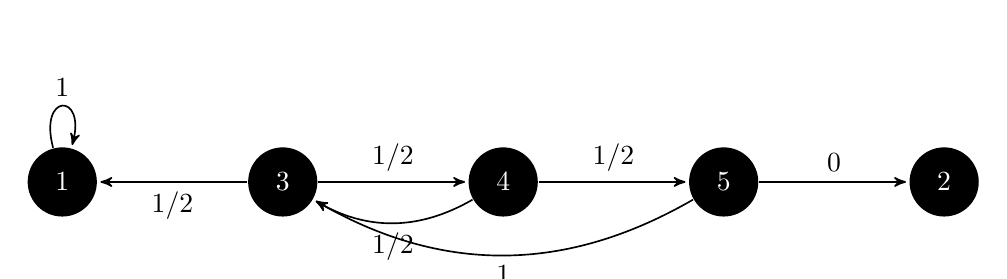
\begin{tikzpicture}[->,>=stealth',shorten >=1pt,auto,node distance=2.8cm,
  semithick]
  \tikzstyle{every state}=[fill=black,draw=none,text=white]

  \node[state]         (A)              {$3$};
  \node[state]         (B) [right of=A] {$4$};
  \node[state]         (C) [left of=A] {$1$};
  \node[state]         (D) [right of=B] {$5$};
  \node[state]         (E) [right of=D] {$2$};

  \path (A) edge              node {1/2} (B)
        (A) edge              node {1/2} (C)
        (B) edge [bend left]  node {1/2} (A)
        (B) edge              node {1/2} (D)
        (C) edge [loop above] node {1} (C)
        (D) edge [bend left]  node {1} (A)
        (D) edge              node {0} (E)
        ;
\end{tikzpicture}

\subsection{}

\begin{subequations}
  \begin{align}
    p'_{34} &= P(X(n)=4|X(n-1)=3,X(\infty)=1)\\
            &= \frac{1}{2}\frac{4}{5}\\
            &= \frac{2}{5}
  \end{align}
\end{subequations}

\begin{subequations}
  \begin{align}
    p'_{35} &= P(X(n)=5|X(n-1)=3,X(\infty)=1)\\
            &= \frac{1}{4}\frac{2}{5}\\
            &= \frac{1}{10}
  \end{align}
\end{subequations}

\begin{subequations}
  \begin{align}
    p'_{35} &= P(X(n)=5|X(n-1)=3,X(\infty)=1)\\
            &= \frac{1}{4}\frac{2}{5}\\
            &= \frac{1}{10}
  \end{align}
\end{subequations}

\begin{subequations}
  \begin{align}
    p'_{43} &= P(X(n)=3|X(n-1)=4,X(\infty)=1)\\
            &= \frac{1}{2}\frac{3}{5}\\
            &= \frac{3}{10}
  \end{align}
\end{subequations}

\begin{subequations}
  \begin{align}
    p'_{45} &= P(X(n)=5|X(n-1)=4,X(\infty)=1)\\
            &= \frac{1}{2}\frac{2}{5}\\
            &= \frac{1}{10}
  \end{align}
\end{subequations}



\begin{subequations}
  \begin{align}
    p'_{i2} =  P(X(n)=2|X(n-1)=i,X(\infty)=1) = 0
  \end{align}
\end{subequations}



\end{document}

